   \documentclass[a4paper,14pt]{extarticle}
\usepackage[utf8]{inputenc}
\usepackage[russian]{babel}
\usepackage{graphicx}
\usepackage[top=0.8in, bottom=0.8in, left=0.8in, right=0.8in]
{geometry}
\usepackage{pgfplots}
\usepackage{amsmath}
\usepackage{setspace}
\usepackage{titlesec}
\usepackage{float}
\usepackage{chngcntr}
\usepackage{pgfplots}
\usepackage{amsfonts}
\usepackage{pgfplotstable}
\usepackage{multirow}
\usepackage{karnaugh-map}
\usepackage{tikz,xcolor}
\usepackage{indentfirst} % Красная строка
\usepackage{listings}
\usepackage{amssymb}
\usepackage{xcolor}
\usepackage{hyperref}

\definecolor{linkcolor}{HTML}{0000FF} % цвет ссылок
\definecolor{urlcolor}{HTML}{FF00FF} % цвет гиперссылок

\hypersetup{pdfstartview=FitH, linkcolor=linkcolor,urlcolor=urlcolor, colorlinks=true}


\titleformat{\section}[hang]
  {\bfseries}
  {}
  {0em}
  {\hspace{-0.4pt}\large \thesection\hspace{0.6em}}
  
  
\titleformat{\subsection}[hang]
  {\bfseries}
  {}
  {0em}
  {\hspace{-0.4pt}\large \thesubsection\hspace{0.6em}}

%\linespread{1.3} % полуторный интервал
%\renewcommand{\rmdefault}{ftm} % Times New Roman

\newcommand{\nx}{\overline{x}}
\newcommand{\p}{0.31}
\newcommand{\scale}{1.4}

\counterwithin{figure}{section}
\counterwithin{equation}{section}
\counterwithin{table}{section}

\begin{document}
\begin{titlepage}
\centering
Санкт-Петербургский политехнический университет Петра Великого \\
\vspace{0.15cm}
Кафедра компьютерных систем и программных технологий \\
\vspace{6.5cm}

{\centering \textbf{Отчёт по лабораторной работе} \\ 
\vspace{0.15cm}
\textbf{Дисциплина}: Телекоммуникационные технологии \\
\vspace{0.15cm}
\textbf{Тема}: Линейная фильтрация} \\


\vspace{6.5cm}

\begin{table}[H]
\begin{tabular}{p{\textwidth}@{}r}
{Выполнил студент гр. 33501/4} \hfill {Мальцев  М.С.} \\
{Преподаватель} \hfill {Богач Н.В.} \\
\end{tabular}
\end{table}
\vfill

{\centering Санкт-Петербург \\ 
\vspace{0.15cm}
\today}
\end{titlepage}

\tableofcontents
\newpage

\section{Цель работы}

Изучить воздействие ФНЧ на тестовый сигнал с шумом.

\section{Постановка задачи}

Сгенерировать гармонический сигнал с шумом
и синтезировать ФНЧ. Получить сигнал во временной и частотной областях до и после фильтрации. Сделать выводы о воздействии ФНЧ на спектр сигнала.

\section{Теоретический раздел}

\subsection{Цифровые фильтры}

Цифровой фильтр — в электронике любой фильтр, обрабатывающий цифровой сигнал с целью выделения и/или подавления определённых частот этого сигнала. В отличие от цифрового, аналоговый фильтр имеет дело с аналоговым сигналом, его свойства недискретны, соответственно передаточная функция зависит от внутренних свойств составляющих его элементов.

Цифровые фильтры на сегодняшний день применяются практически везде, где требуется обработка сигналов, в частности в спектральном анализе, обработке изображений, обработке видео, обработке речи и звука и многих других приложениях.

\subsubsection{Линейность и стационарность цифровых фильтров}

Линейными называются системы, для которых справедлив принцип суперпозиции: сумма эффектов от отдельных воздействий равна эффекту от суммы воздействий. С точки зрения спектральных свойств линейность означает отсутствие на выходе цифровых фильтров гармоник, не присутствовавших во входном сигнале. Стационарность означает постоянство характеристик системы во времени: в стационарной системе произвольная задержка входного сигнала приводит только к такой же задержке выходного сигнала и не меняет его формы. Если это условие не выполняется, система называется нестационарной, параметрической, или системой с переменными параметрами.

\subsubsection{КИХ фильтры}
Фильтр с конечной импульсной характеристикой (нерекурсивный фильтр, КИХ-фильтр) — один из видов линейных цифровых фильтров, характерной особенностью которого является ограниченность по времени его импульсной характеристики (с какого-то момента времени она становится точно равной нулю). 

КИХ-фильтр обладает рядом полезных свойств, из-за которых он иногда более предпочтителен в использовании, чем БИХ-фильтр. Вот некоторые из них:
\begin{enumerate}
\item КИХ-фильтры устойчивы.
\item КИХ-фильтры при реализации не требуют наличия обратной связи.
\item Фаза КИХ-фильтров может быть сделана линейной
\end{enumerate}

\subsubsection{БИХ фильтры}
фильтр с бесконечной импульсной характеристикой (Рекурсивный фильтр, БИХ-фильтр) или IIR-фильтр — линейный электронный фильтр, использующий один или более своих выходов в качестве входа, то есть образующий обратную связь. Основным свойством таких фильтров является то, что их импульсная переходная характеристика имеет бесконечную длину во временной области, а передаточная функция имеет дробно-рациональный вид. Такие фильтры могут быть как аналоговыми, так и цифровыми.

Примерами БИХ-фильтров являются фильтр Чебышёва, фильтр Баттерворта, Фильтр Калмана и фильтр Бесселя.

Об устойчивости фильтра с бесконечной импульсной характеристикой судят по его передаточной функции. Для дискретного фильтра необходимо и достаточно, чтобы все полюса его передаточной функции по модулю были меньше единицы (т.е. лежали внутри единичного круга на z-плоскости). Все критерии устойчивости, применимые в теории линейных стационарных систем, например критерий устойчивости Найквиста или критерий устойчивости Рауса применимы и в случае БИХ-фильтров.

В отличие от КИХ-фильтров, БИХ-фильтры не всегда являются устойчивыми.

\section{Ход работы}

\subsection{Исследование предсозданой модели фильтра в Simulink}

При открытие Simulink оказалось, что в нём имеются примеры применения фильтров.

\begin{figure}[H]
\center{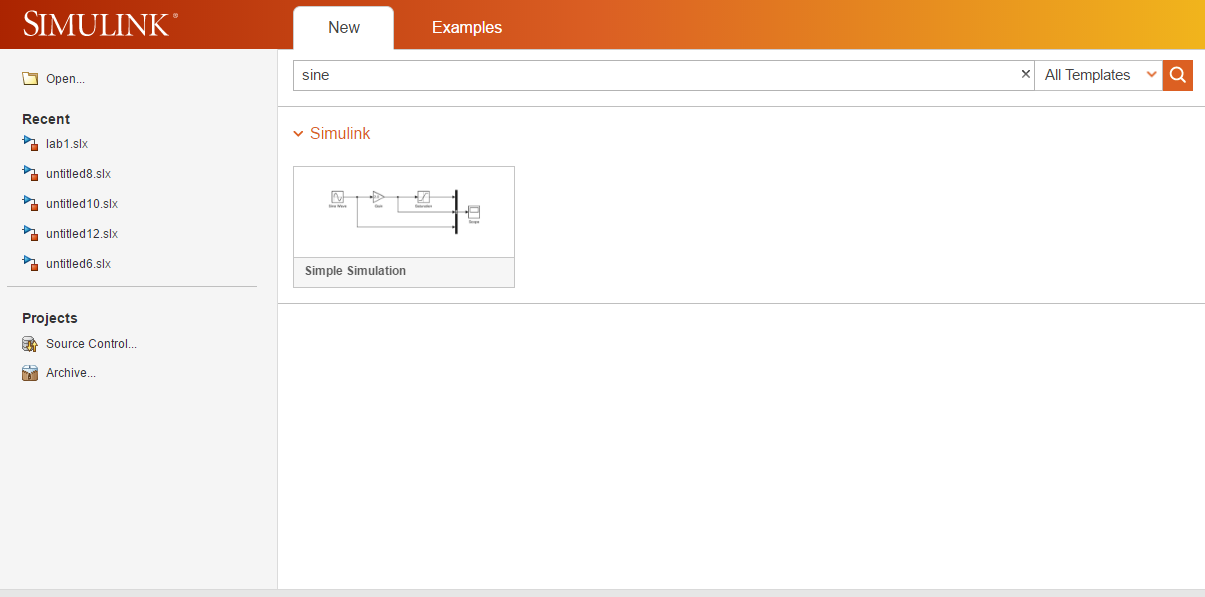
\includegraphics[width=1\linewidth]{img/000.png}}
\caption{Шаблоны для построения фильтров. Окно Simulink Start Page.}
\label{000}
\end{figure}

Был выбран шаблон "Digittal Filter".

\begin{figure}[H]
\center{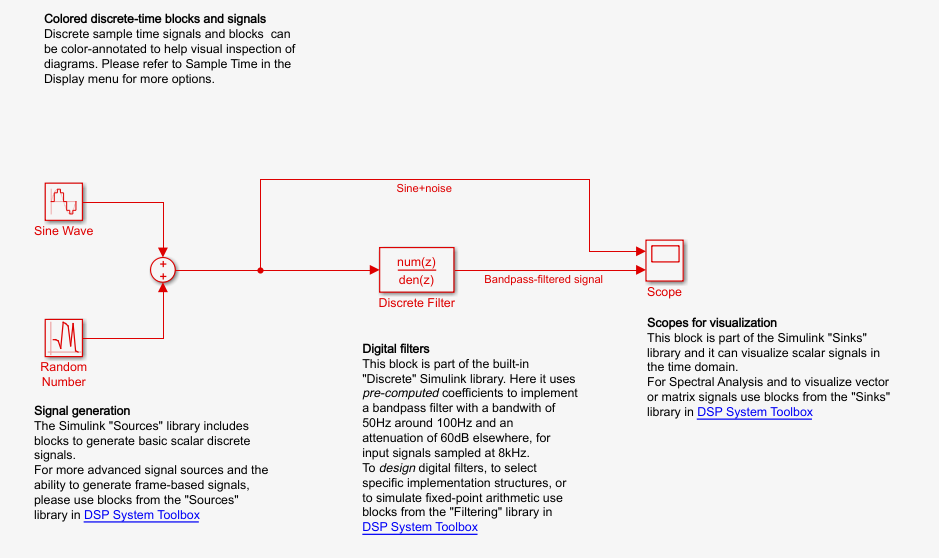
\includegraphics[width=0.9\linewidth]{img/001.png}}
\caption{Шаблон "Digittal Filter".}
\label{001}
\end{figure}

На изображении \ref{001} видно, что происходит объединение двух сигналов: синусоидального и случайного и мы получаем зашумленный синусоидальный сигнал. Далее применяется фильтрация и шум отделяется от основного сигнала.
 
После стара симуляции, было получено изображение \ref{002}.

\begin{figure}[H]
\center{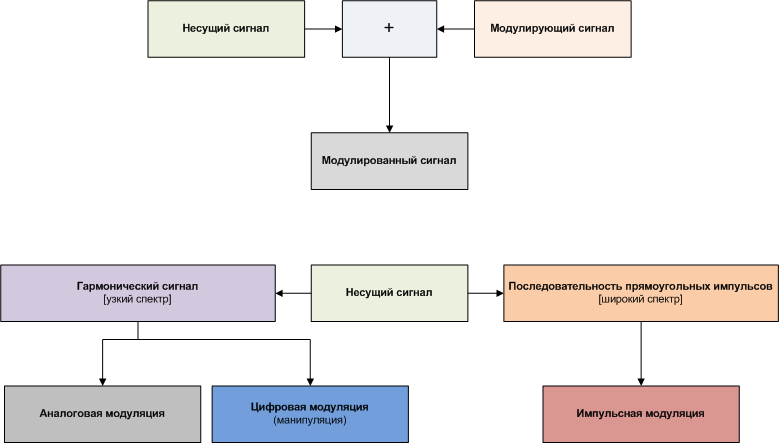
\includegraphics[width=1\linewidth]{img/002.png}}
\caption{Результат симуляции шаблона "Digittal Filter".}
\label{002}
\end{figure}

На рисунке \ref{002} видно, что два сигнала: один -- зашумлённый синусоидальный сигнал (обозначен жёлтым), другой -- отфильтрованный от шума (обозначен бирюзовым).


\subsection{Создание собственного фильтра и его исследование на зашумленном сигнале}

\subsubsection{Создание зашумленного сигнала}

Была разработана схема, в которой к синусоидальному сигналу добавляется белый шум. Схема продемонстрирована на рисунке \ref{003}.

\begin{figure}[H]
\center{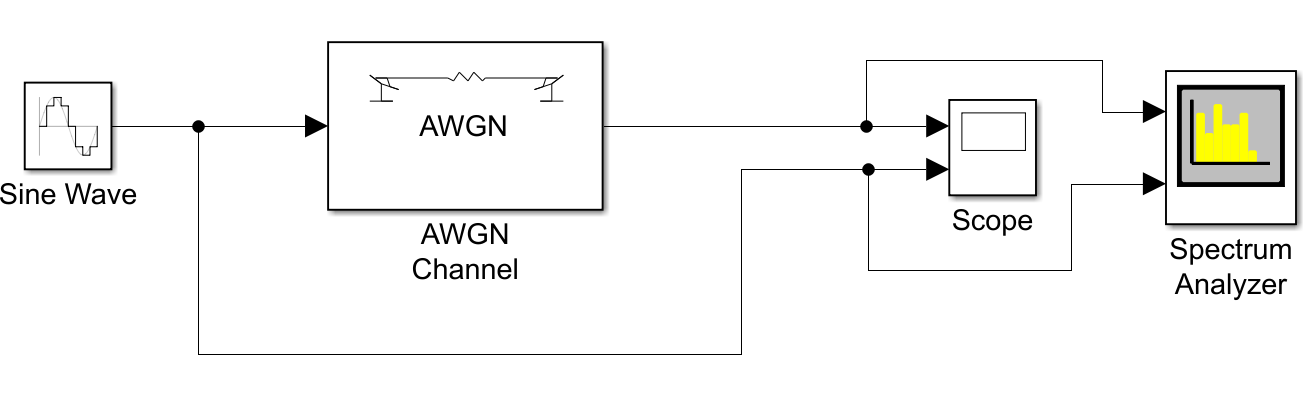
\includegraphics[width=1\linewidth]{img/003.png}}
\caption{Схема разработанная в Simulink.}
\label{003}
\end{figure}

Для элементов $Sin \ Wave$ и $AWGN \ Channel$ были заданы параметры, продемонстрированные на рисунке \ref{003_12}.

\begin{figure}[h]
\begin{minipage}[h]{0.49\linewidth}
\center{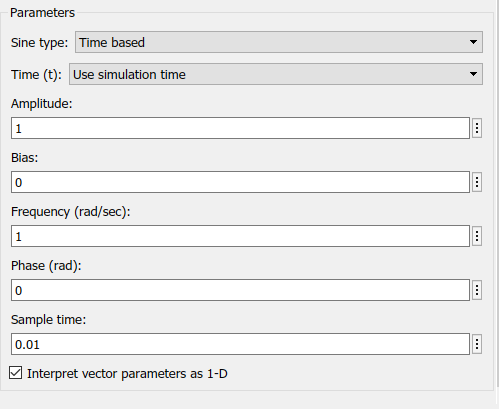
\includegraphics[width=1\linewidth]{img/003_1.png} \\ а) для элемента Sin Wave}
\end{minipage}
\hfill
\begin{minipage}[h]{0.49\linewidth}
\center{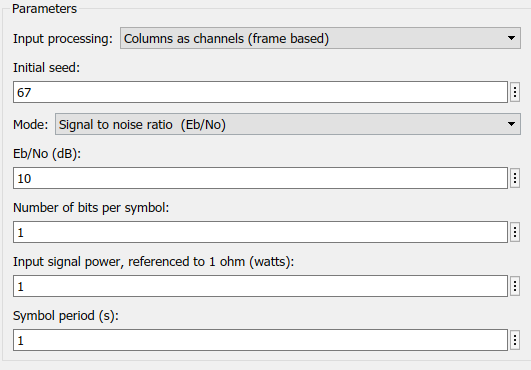
\includegraphics[width=1\linewidth]{img/003_2.png} \\ б) для элемента AWGN Channel }
\end{minipage}
\caption{Параметры для элементов $Sin \ Wave$ и $AWGN \ Channel$.}
\label{003_12}
\end{figure}

Была проведена симуляция. Результат представлен на рисунках \ref{004} и \ref{005}.

\begin{figure}[H]
\center{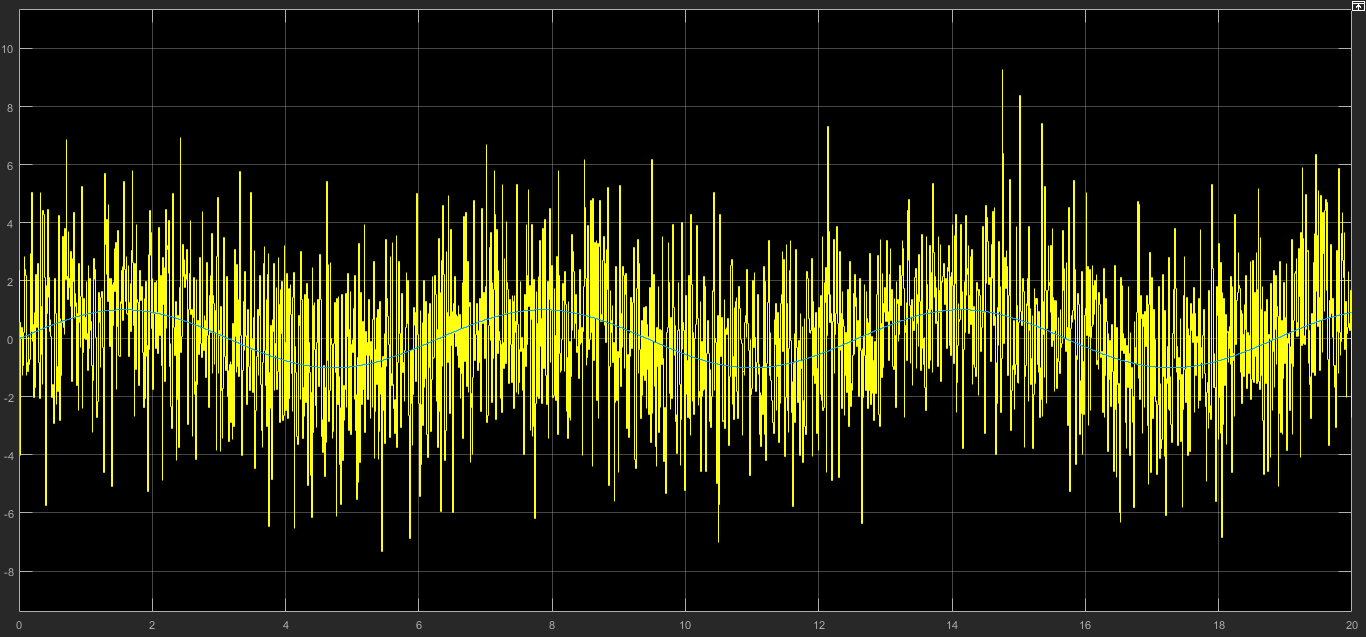
\includegraphics[width=1\linewidth]{img/004.png}}
\caption{Исходный и зашумленный сигналы во временной области.}
\label{004}
\end{figure}

На рисунке \ref{004} видно, что на исходный сигнал(обозначен бирюзовым цветом) наложен шум. Причём, достаточно сложно визуально отделить исходный сигнал от зашумлённого.

\begin{figure}[H]
\center{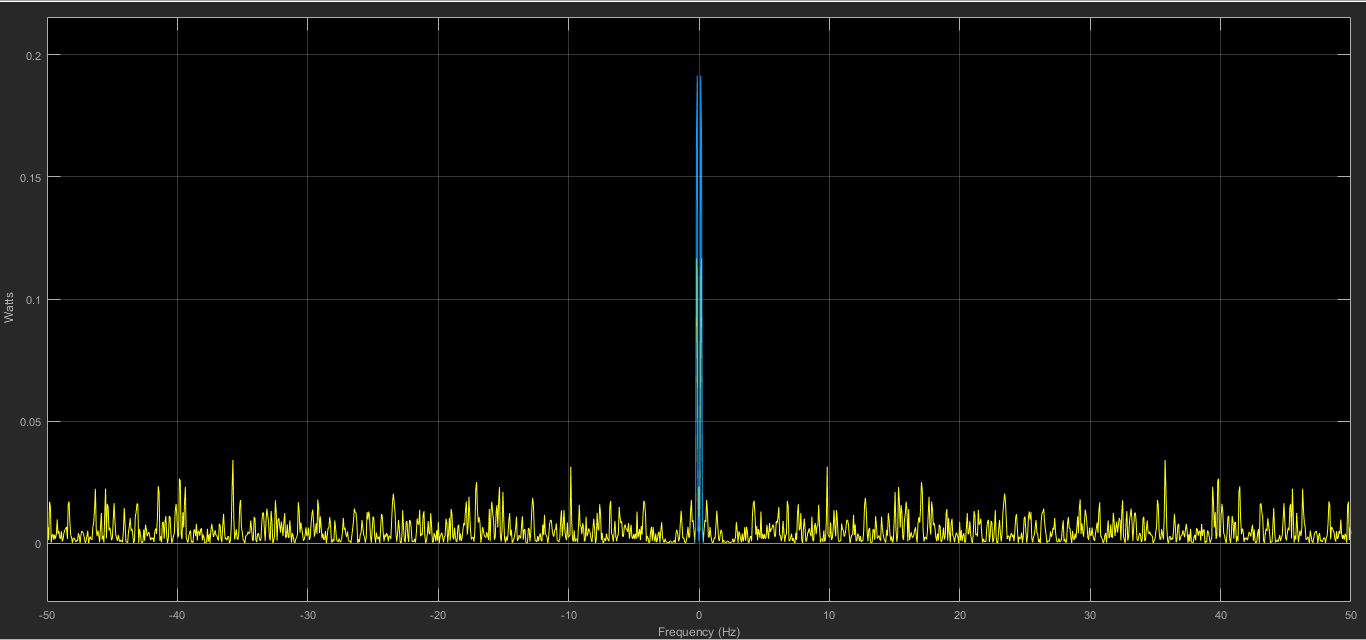
\includegraphics[width=1\linewidth]{img/005.png}}
\caption{Спектры исходного и зашумленного сигналов.}
\label{005}
\end{figure}

\begin{figure}[H]
\center{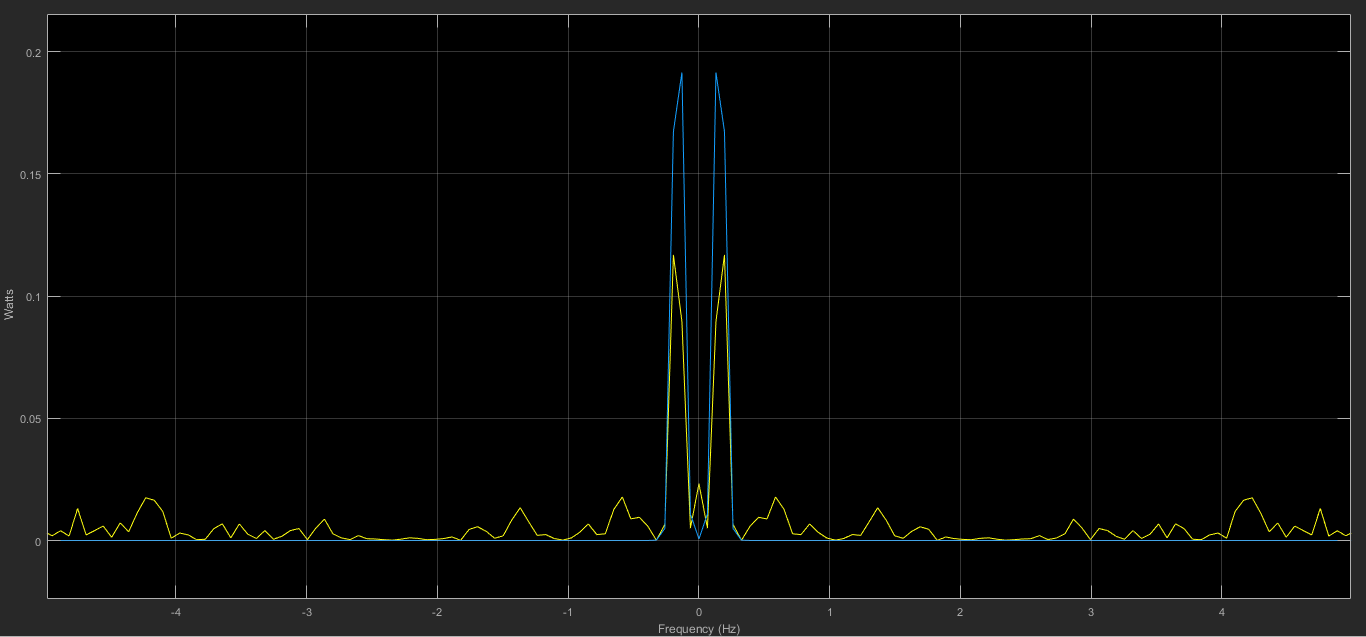
\includegraphics[width=1\linewidth]{img/005_1.png}}
\caption{Спектры исходного и зашумленного сигналов.}
\label{005_1}
\end{figure}

На рисунках \ref{005} и \ref{005_1} отчётливо различаются основной сигнал и шум, добавленный к нему. Заметим, что амплитуда сигнала после зашумления уменьшилась.

\subsubsection{Создание собственного фильтра}

Схема представленная на рисунке \ref{003} была модифицирована. Изменённая схема представлена на рисунке \ref{006}.

\begin{figure}[H]
\center{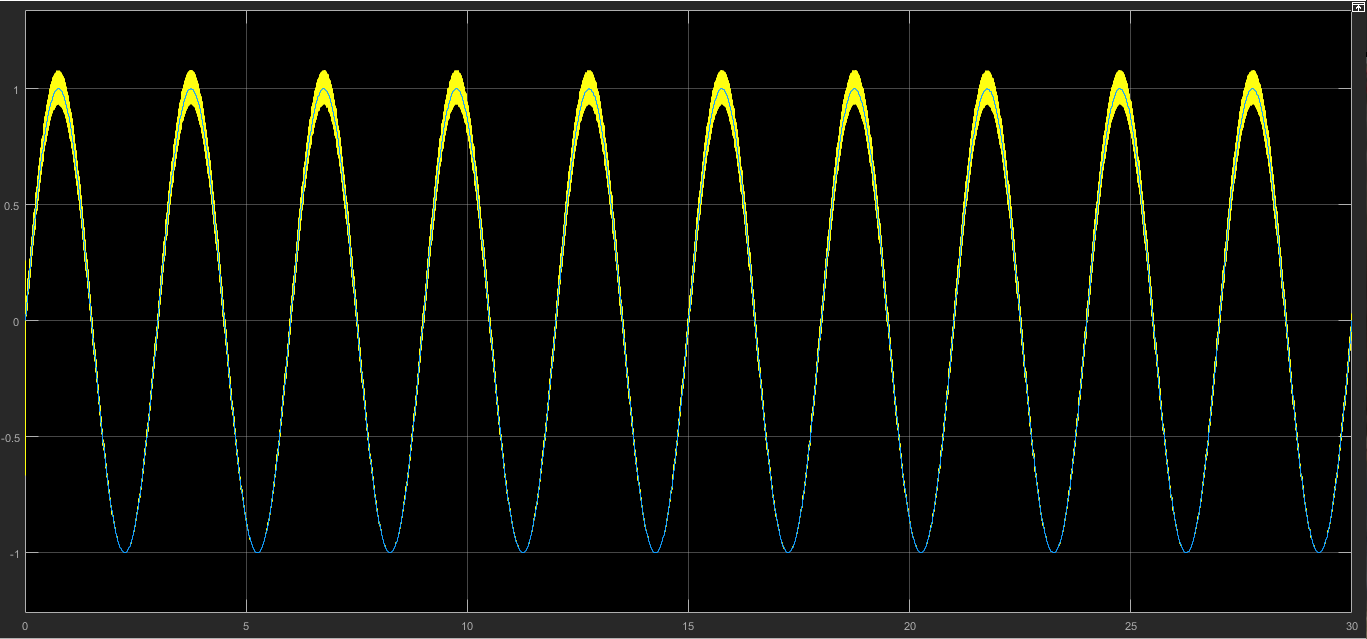
\includegraphics[width=1\linewidth]{img/006.png}}
\caption{Модифицированная схема для исследования фильтра.}
\label{006}
\end{figure}

\begin{figure}[H]
\center{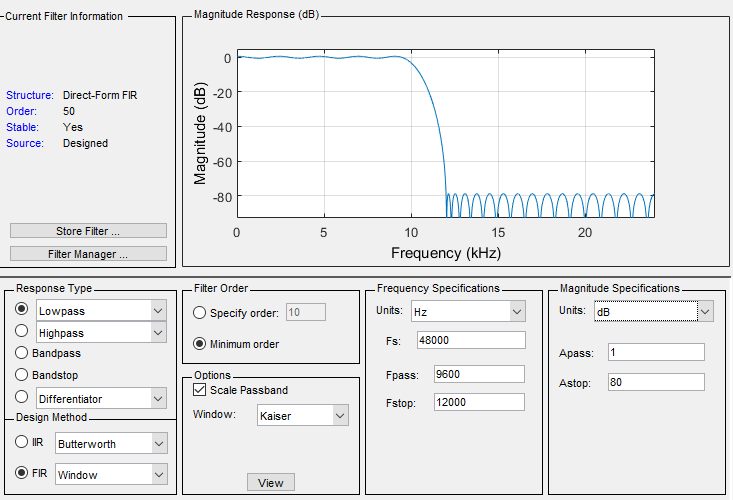
\includegraphics[width=1\linewidth]{img/006_1.png}}
\caption{Параметры элемента $Filter$.}
\label{006_1}
\end{figure}

Не изменяя начальных параметров фильтра, запустим симуляцию. Полученные результаты продемонстрированы на рисунке \ref{007}.

\begin{figure}[H]
\center{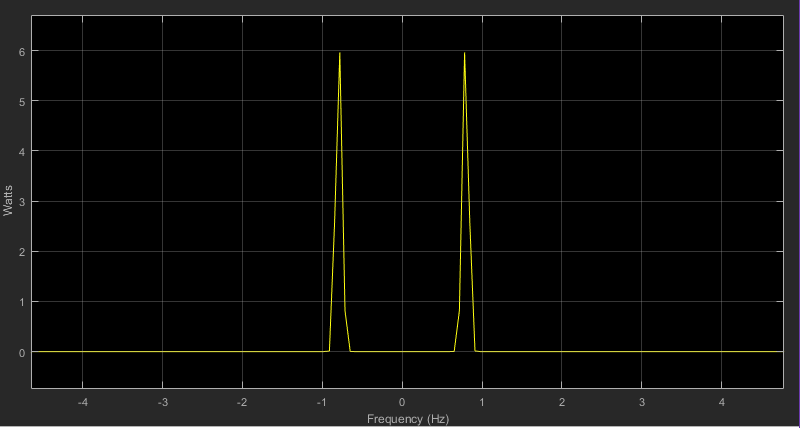
\includegraphics[width=1\linewidth]{img/007.png}}
\caption{Спектры зашумленного сигнала до и после применения фильтра.}
\label{007}
\end{figure}

Изменим параметры фильтра(рисунок \ref{008}) и посмотрим, к каким последствиям это привело. Результаты симуляции проведены на рисунке \ref{009}.

\begin{figure}[H]
\center{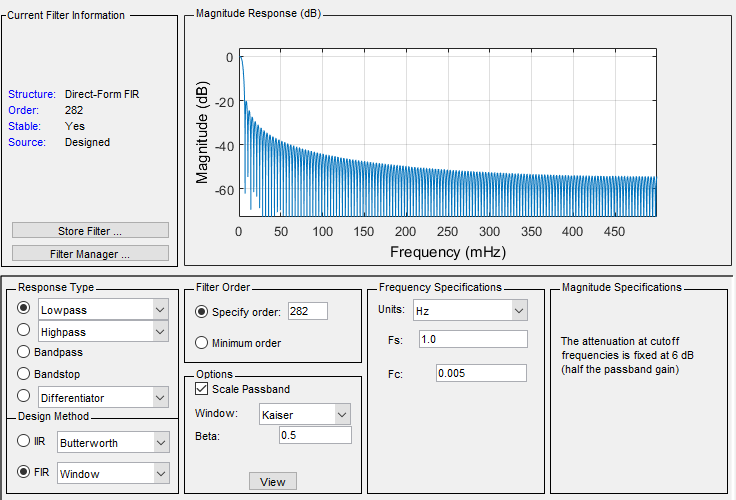
\includegraphics[width=1\linewidth]{img/008.png}}
\caption{Параметры элемента $Filter$.}
\label{008}
\end{figure}

\begin{figure}[H]
\center{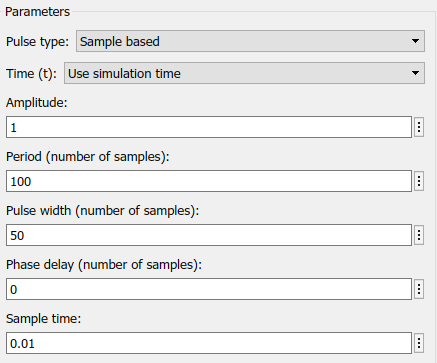
\includegraphics[width=1\linewidth]{img/009.png}}
\caption{Спектры зашумленного сигнала до и после применения фильтра.}
\label{009}
\end{figure}

Итог: исходный сигнал успешно выделен, шум удалён фильтром.
Результат во временной области, рисунок \ref{010}.

\begin{figure}[H]
\center{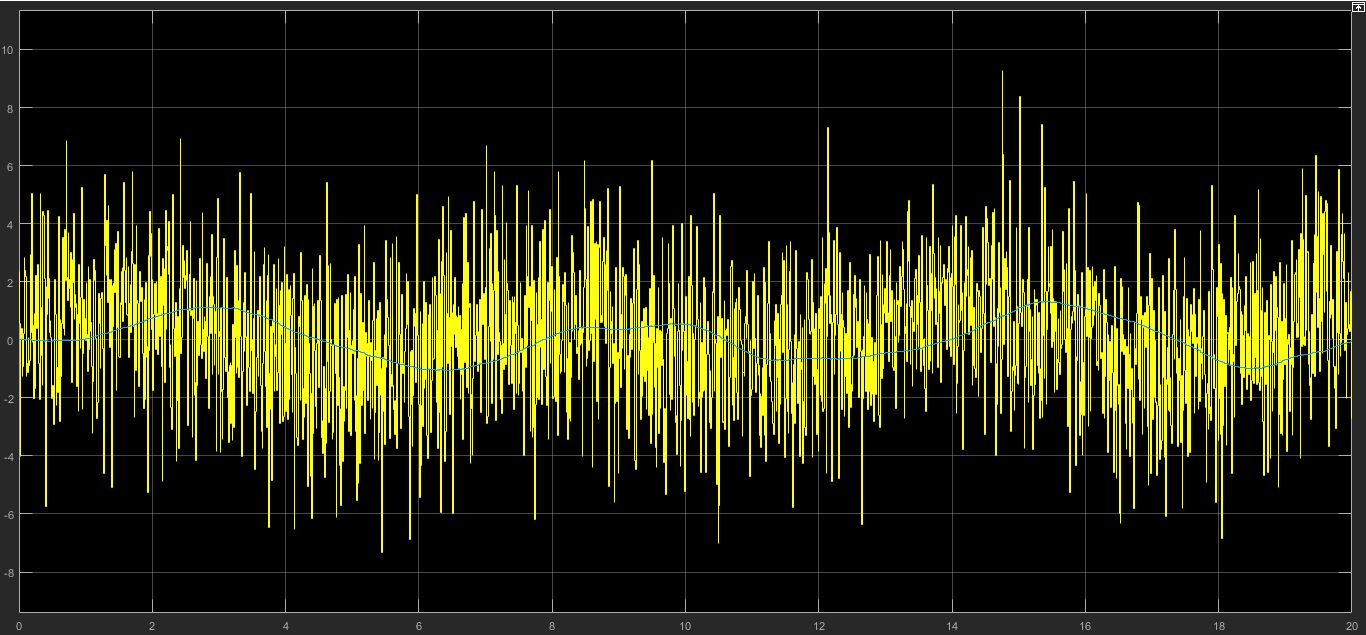
\includegraphics[width=1\linewidth]{img/010.png}}
\caption{Зашумленный сигнал во временной области до и после применения фильтра.}
\label{010}
\end{figure}

Визуально сравним исходный сигнал и сигнал, к которому мы добавили шум и отфильтровали. Для этого воспользуемся рисунками

\begin{figure}[H]
\center{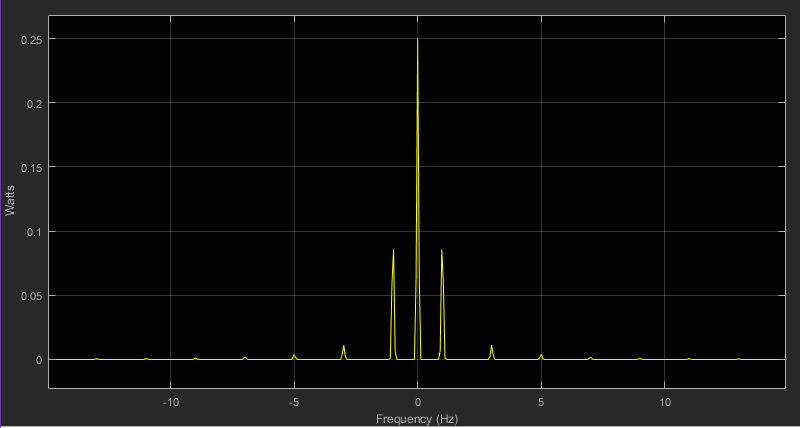
\includegraphics[width=1\linewidth]{img/011.png}}
\caption{Исходный сигнал и сигнал полученный после фильтрации зашумленного, во временной области.}
\label{011}
\end{figure}

\begin{figure}[H]
\center{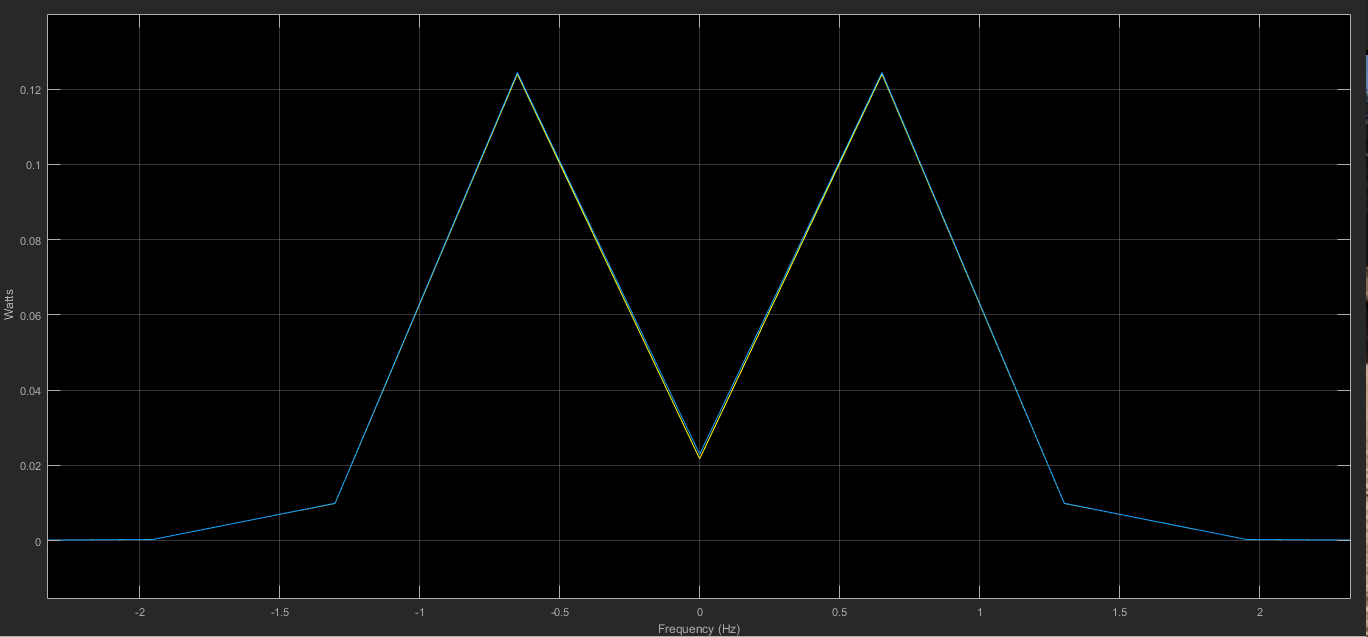
\includegraphics[width=1\linewidth]{img/012.png}}
\caption{Исходный сигнал и сигнал полученный после фильтрации зашумленного, в частотной области.}
\label{012}
\end{figure}

По полученным результатам можно сделать вывод, что фильтр работает удовлетворительно, так как отфильтрованный зашумленный сигнал соответствует исходному.



\section{Выводы}

При прохождении сигнала через линейный фильтр, спектр сигнала на его выходе получается путём умножения спектра входного сигнала на частотную характеристику фильтра. Для временной области получаем, что выходной сигнал после линейного фильтра соответствует свертке сигнала с импульсной характеристикой фильтра. 

В ходе работы был исследован фильтр из примера библиотеки $Simulink$, а также создана собственная схема для генерации синусоидального сигнала, зашумления его и дальнейшей фильтрации. Отфильтрованный сигнал визуально почти соответствует исходному, что свидетельствует от правильной настройке фильтра. Но в то же время, сигнал полученный после фильтрации несколько искажен -- это связано с тем, что белый шум распределён по всем частотам, следовательно, он существует и на тех, что и исходный сигнал, что его искажает.

\section{Используемые материалы}

\begin{enumerate}

\item \href{http://www.kit-e.ru/articles/cad/2009_05_127}{Синтез цифровых фильтров в $Matlab$}

\item \href{https://vunivere.ru/work11332}{Чья-то лабораторная, которая продаётся}

\item \href{https://en.wikipedia.org/wiki/Digital_filter}{Digital filter (Wikipedia)}

\item \href{http://present5.com/cifrovye-filtry-chast-1-linejnost-i-stacionarnost/}{Презентация "Цифровые фильтры"}

\end{enumerate}

\end{document}